\section{연구 결과}

\subsection{GS-touch 컨트롤러 하드웨어 제작}

Fig. \ref{fig:final_product_How_it_works_big}\는 최종 완성된 GS-touch 하드웨어와 GS-touch\가 동작하는 원리를  나타낸 것이다. PCB를 제작하여 부품을 하나하나 납땜하여 기판을 완성하였고, 3D 프린터를 이용하여 케이스를 출력하여 조립하였다. 전체적인 모양이나 크기 등 일부 개선할 부분이 있으나 사용하는데 큰 지장은 없다.

\begin{figure}[H]
	\begin{center}
		\begin{tikzpicture}
		\node[anchor=south west,inner sep=0] at (0,0) {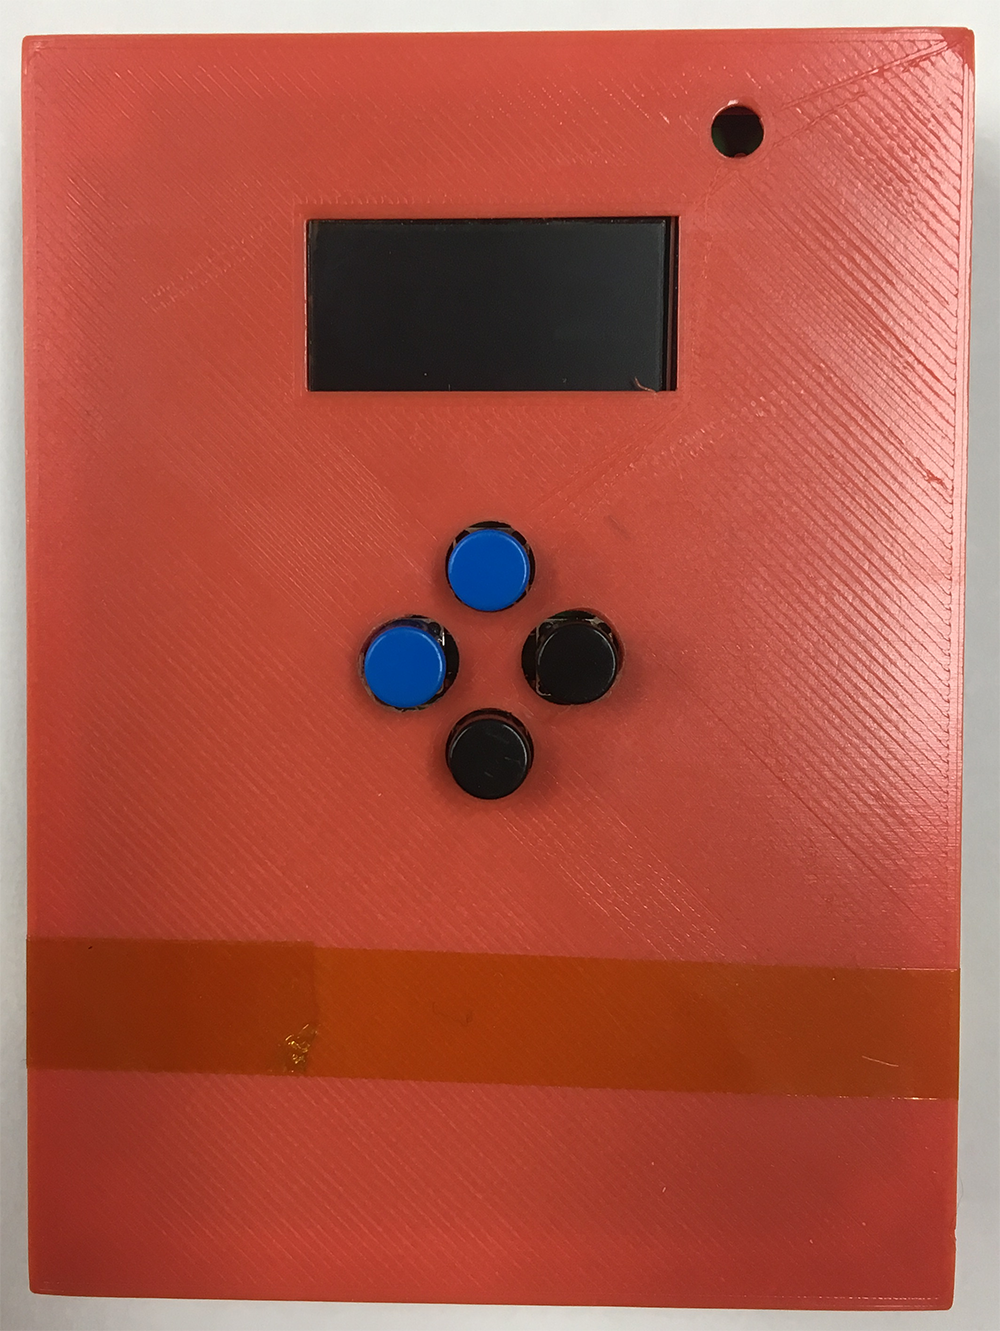
\includegraphics[width=0.32\linewidth]{GS-touch_final} 
		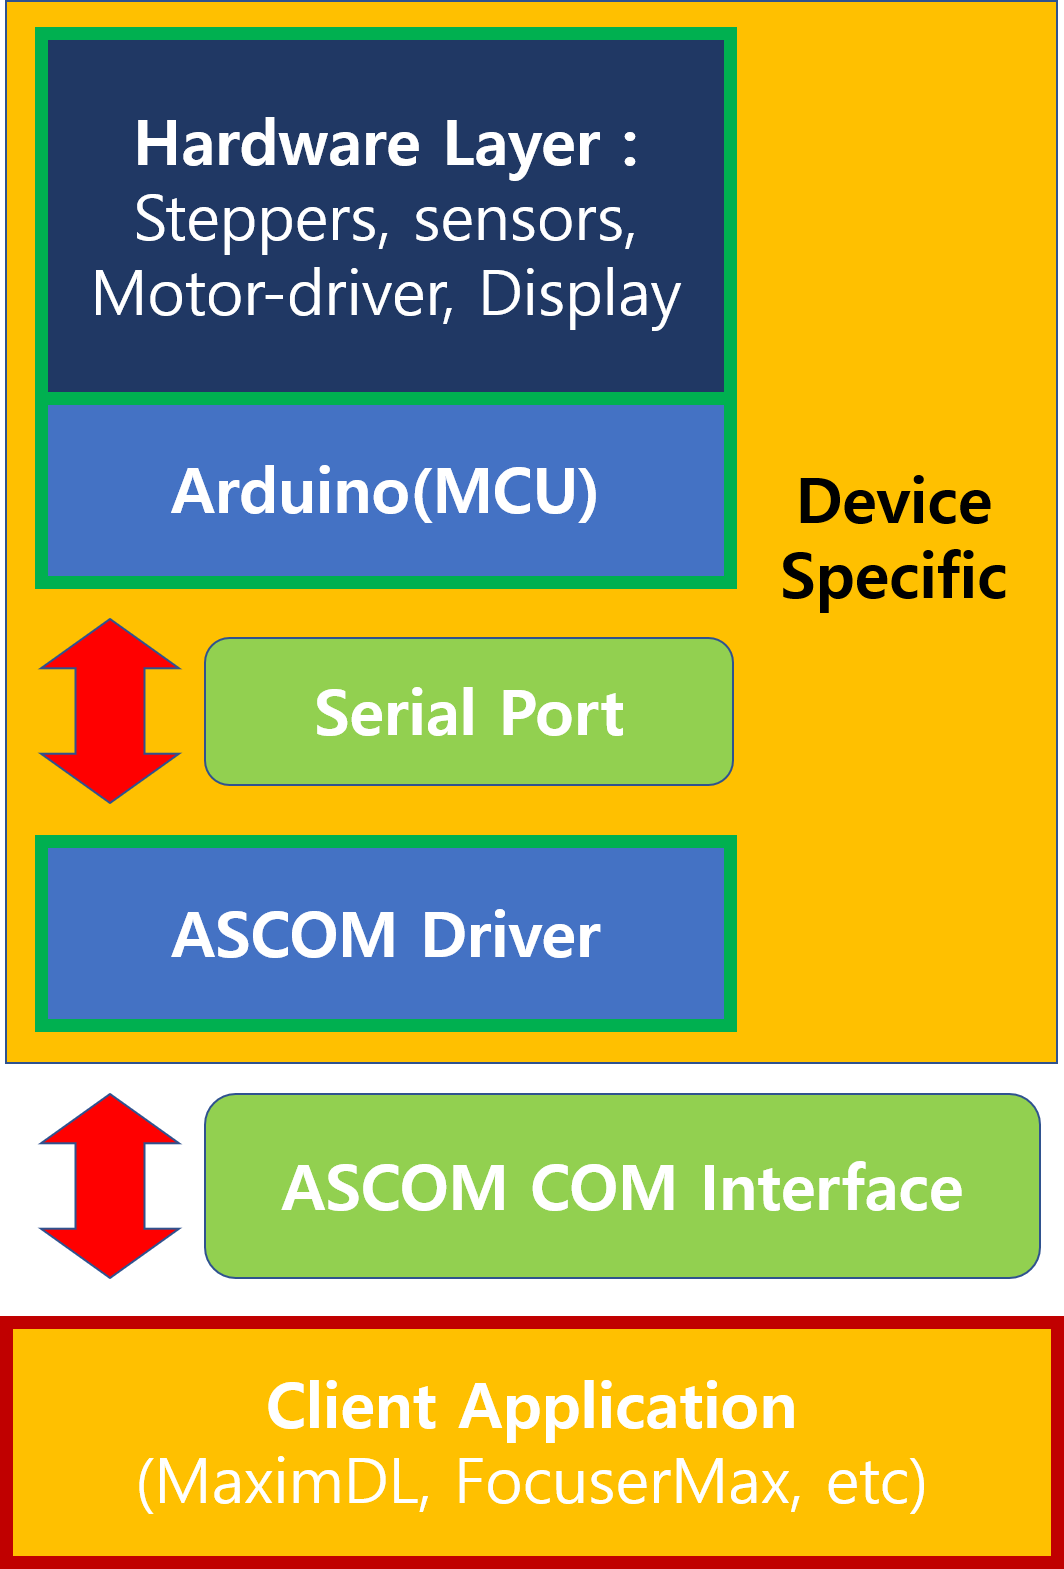
\includegraphics[width=0.29\linewidth]{How_it_works_big}};
		\draw[text=black] (0.2, 7.3) node {(a)};
		\draw[text=black] (5.7, 7.3) node {(b)};
		\end{tikzpicture}
		\caption{(a) GS-touch 하드웨어와 (b) GS-touch 동작 원리}
	\label{fig:final_product_How_it_works_big}
	\end{center}
\end{figure}

\subsection{GS-touch 펌웨어 개발}

개발된 기반 펌웨어는 컴퓨터와 다르게 지정된 디스플레이어 에만 표시를 할 수 있다는 특징이 있다. 따라서 여러 가지 기능이 존재하더라도 한번에 여러 가지의 동작을 진행할 수는 없다. 그렇기 때문에 모터를 움직이는 여러 명령들을 효율적으로 처리하기 위해 하드웨어에 탑재된 버튼을 이용하여 이동과 선택이 쉬운 메뉴와 서브 메뉴를 만들어 사용하는 방식을 택하여 핵심 기능들이 모두 펌웨어에 들어갈 수 있도록 하였다.

\begin{figure}[h]
	\begin{center}
		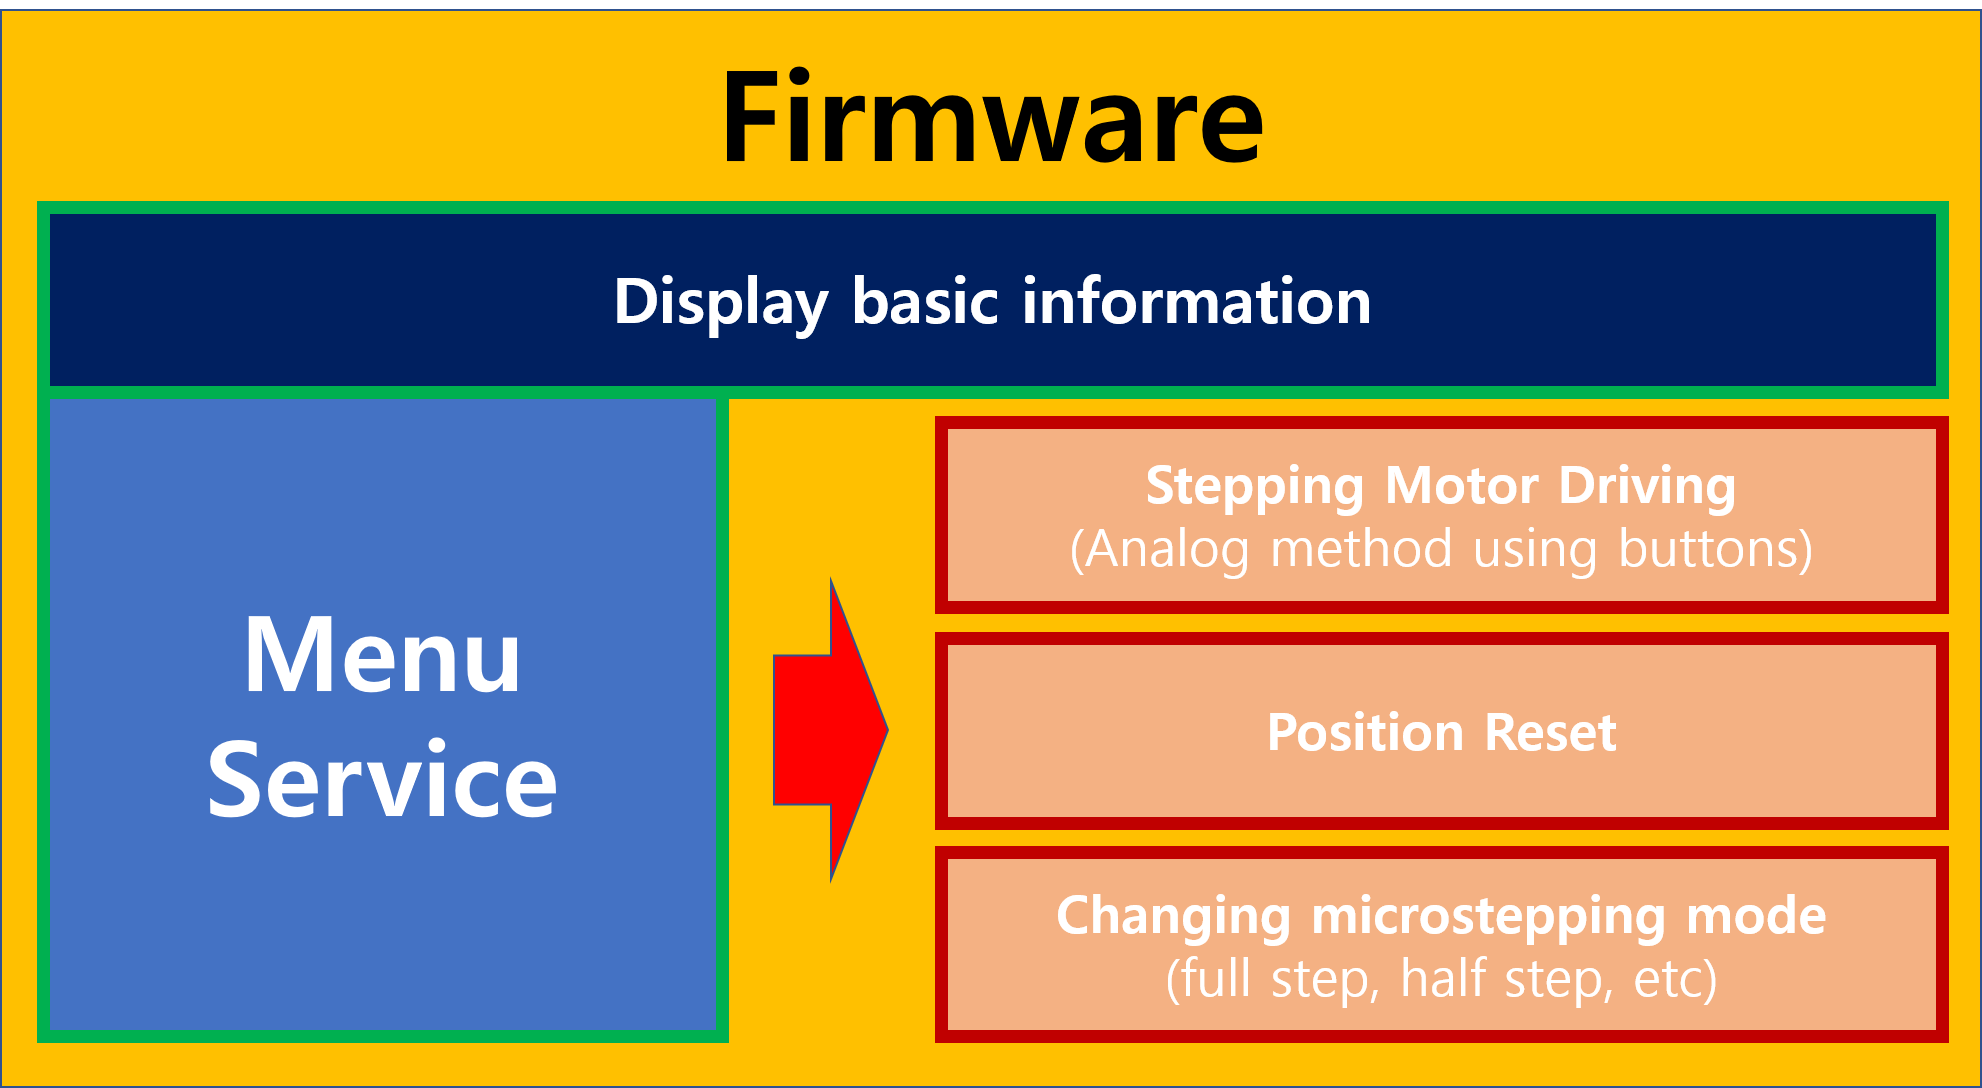
\includegraphics[width=0.6\linewidth]{firmware_big}
	\end{center}
	\caption{펌웨어에 구현된 핵심 기능}
	\label{fig:firmware_big}
\end{figure}

펌웨어의 첫 번째 기능은 모터 초점 조절 장치의 핵심이라고도 할 수 있는 기능으로, 앞서 설명하였듯이 스테핑 모터를 조절하는 데 있어 가장 중요한 것은 정확한 스텝으로 정확한 각도를 이동하는 것이다. 즉, 제작한 펌웨어에는 현재 스테핑 모터의 각도를 나타내는 정보(position)를 나타낼 수 있으며, 버튼을 이용하여 아주 작은 간격(single step)으로 모터의 각도를 이동할 수 있도록 하였다.

장치를 사용하다보면 제공되는 최대 스텝수가 부족하거나 현재 위치를 기억해야 할 때가 있다. 이럴 때 필요한 기능이 position을 원하는 곳으로 초기화하는 것이다. 예를 들어, 대부분의 사람들은 포커서가 끝에 위치할 때의 position을 0으로 설정하고 싶을 것이다. 꼭 끝점이 아니더라도 이미 초점을 맞춘 상황을 기준으로 삼고 싶어서 position을 바꾸고 싶을 수 있을 것이다. 이 때 필요한 기능이 position을 지정된 범위 내에서 초기화시키는 것(reset position)이다. 위에서 설명한 상황이 아니더라도 GS-toufocuser을 껏다가 위치를 이동시켰던 경우에도 실제 위치를 기억하지 못할 때도 있을 것이다. 이런 상황에서도 position을 초기화시키는 기능이 사용될 것이다.

부가적인 기능으로, 망원경의 특성의 차이때문에 같은 각도를 이동하더라도 포커서가 이동하는 거리가 달라질 수도 있고, 필요한 힘이 달라지거나 한번에 이동하는 거리가 달라질 수도 있다. 이렇게 필요한 상황에 따라서 적절하게 microstepping을 바꿀 수 있는 기능 또한 펌웨어에 탑재되어있다. 또한, 모터를 움직이는 상황이 아니라면 센서에서 측정된 온도와 습도를 표시할 수 있도록 하였다.

\subsection{ASCOM driver 및 컨트롤 프로그램 개발}

ASCOM 드라이버를 ASCOM Protocol에 맞게 개발하여 여러가지 프로그램 및 망원경 사이의 편의성을 증대시키고자 하였다. ASCOM 드라이버는 직접 띄우는 창을 설정하여 여러가지 상황에 맞는 기능들을 제공할 수 있으며, 컴퓨터의 화면 상에서 일어나기 때문에 비교적 많은 정보를 한번에 표현할 수 있다.

C\#에서 지원하는 파일 형식은 .cs의 이름을 가지고 있으며, ASCOM Protocol에 맞게 작성된 ASCOM 드라이버를 표현하는 프로젝트는 크게 3가지 부분으로 이루어져 있다. Driver.cs 파일, SetupDialogForm.cs 파일, MainWindow.cs 파일이 그 세 가지이며, 각 파일들에서 실행시키는 영역이 모두 다르게 설계되어 있다.

Driver.cs는 serial Port를 이용하여 펌웨어와 직접적으로 통신하는 기능을 가지고 있다. ASCOM 지원 소프트웨어에서 장치를 구동하기 위해서 제일 먼저 해야 하는 일은 장치를 선택하고 통신환경 설정을 하는 것이다. Driver.cs는 ASCOM Setup을 선택할 경우 Fig. \ref{fig:focuserchooser}과 같이 나타나며 GS-touch ASCOM driver 이다. 이 드라이버가 설치되어 있지 않으면 GS-focus를 사용할 수 없다. 이 파일을 가장 중요한 기능은 프로그램이 내릴 수 있는 여러가지 명령을 serial command를 설정하여 각각 실행할 수 있도록 하는 것이다. 만약 서로 다른 프로그램에서 serial Port를 통한 연결(Port를 open한다고 표현한다)을 진행하려고 하면 그동안 진행했던 정보들을 모두 다시 전달해야하기 때문에 복잡한 처리과정을 거쳐야 한다. 때문에 serial Port와 관련된 함수 및 연결을 하나의 파일에서 모두 실행시킬 수 있도록 하였다.

\begin{figure}[h]
	\begin{center}
	\begin{tikzpicture}
	\node[anchor=south west,inner sep=0] at (0,0) {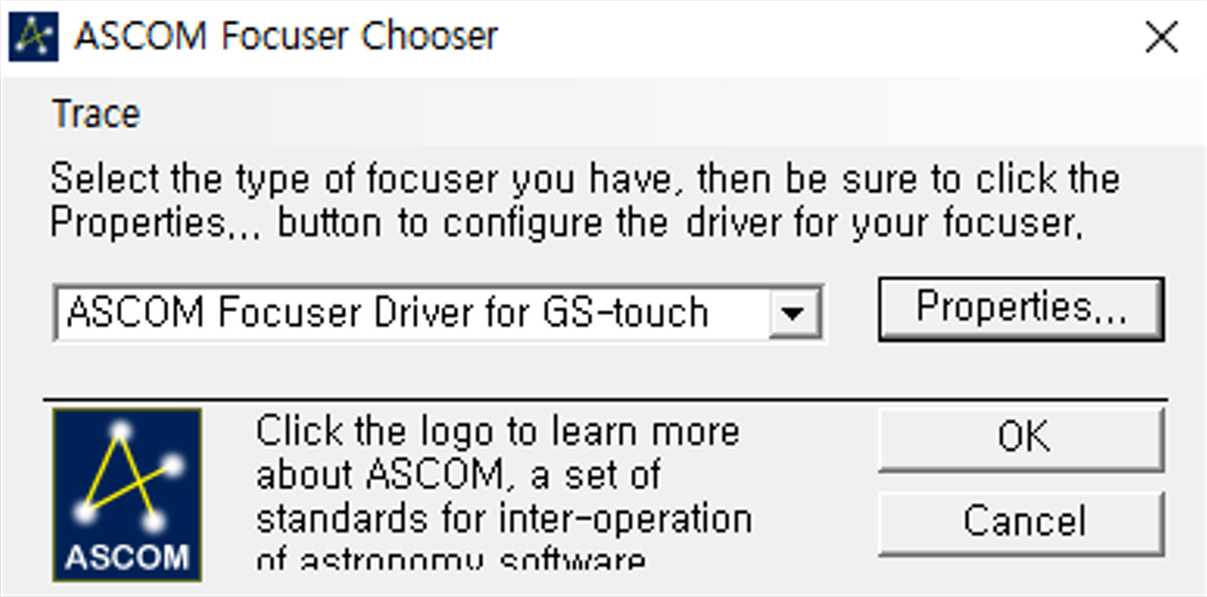
\includegraphics[width=0.6\linewidth]{A_focuserchooser}};
	\draw[draw=red, line width=0.5mm] (0.4, 2.05) rectangle (6.8, 2.61);
	\draw[text=red] (0.1, 2.3) node {(a)};
	\draw[draw=red, line width=0.5mm] (7.2, 2.05) rectangle (9.6, 2.61);
	\draw[text=red] (10.0, 2.30) node {(b)};
	\draw[draw=red, line width=0.5mm] (7.2, 1.04) rectangle (9.6, 1.55);
	\draw[text=red] (10.0, 1.29) node {(c)};
	\draw[draw=red, line width=0.5mm] (7.2, 0.33) rectangle (9.6, 0.84);
	\draw[text=red] (10.0, 0.58) node {(d)};
	\end{tikzpicture}
	\end{center}
	\caption{Focuser chooser windows : (a) choosing focuser, (b) Properties; excute SetupDialogForm.cs, (c) OK; apply results, (d) Cancel; close Form}
\label{fig:focuserchooser}	
\end{figure}

SetupDialogForm.cs는 ASCOM 드라이버를 선택하는 과정에서 직접적으로 연결을 진행하기 전에(직접적인 연결은 Connect를 눌러야 시작된다) 필요한 설정들을 확인하는 절차이다. 이 파일에서는 드라이버와 펌웨어 사이에 연결되어있는 COM port(serial 통신을 하기 위해 usb로 연결되어 있는 포트)를 지정하며, 모터의 microstepping을 설정한다. microstepping설정을 모터를 움직이는 도중에 직접 설정하게 되면 한 스텝당 이동하는 position이 달라지기 때문에 정확한 거리를 계산할 수 없게 되며, 측정을 한 번 진행할 때마다 Position 사이의 거리가 달라진다. 따라서 직접 연결을 진행하기 전에 microstepping을 다시 확인하게 된다.

\begin{figure}[h]
	\begin{center}
		\begin{tikzpicture}
		\node[anchor=south west,inner sep=0] at (0,0) {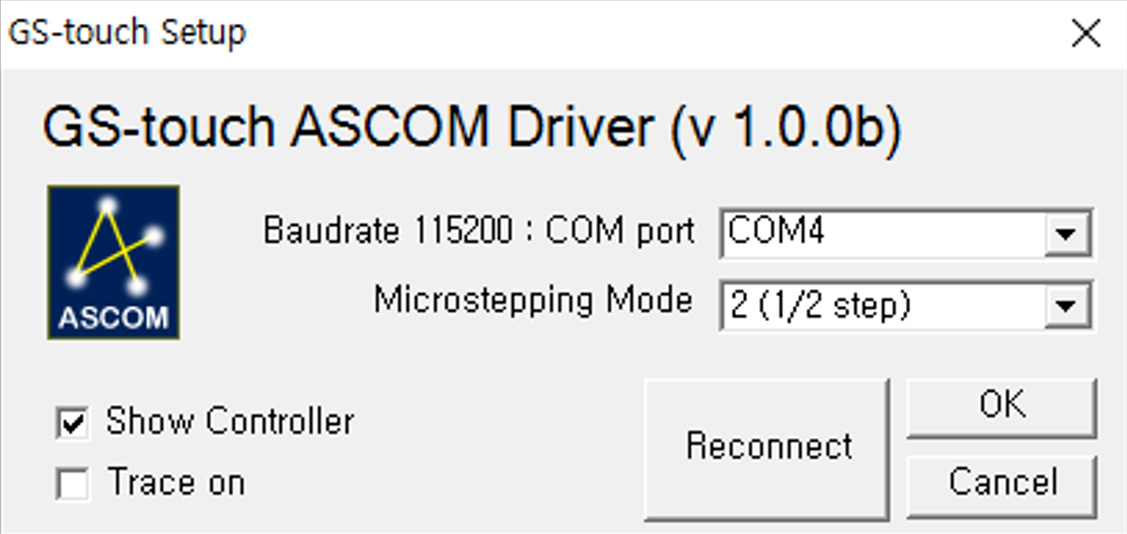
\includegraphics[width=0.6\linewidth]{A_properties}};
		\draw[draw=red, line width=0.5mm] (0.4, 0.7) rectangle (3.20, 1.2);
		\draw[text=red] (0.10, 0.95) node {(a)};
		\draw[draw=red, line width=0.5mm] (0.4, 0.15) rectangle (3.2, 0.65);
		\draw[text=red] (0.10, 0.40) node {(b)};
		\draw[draw=red, line width=0.5mm] (9.8, 2.4) rectangle (6.4, 2.9);
		\draw[text=red] (10.2, 2.6) node {(c)};
		\draw[draw=red, line width=0.5mm] (9.8, 1.75) rectangle (6.4, 2.25);
		\draw[text=red] (10.2, 2.05) node {(d)};
		\draw[draw=red, line width=0.5mm] (7.8, 0.1) rectangle (5.65, 1.4);
		\draw[text=red] (5.3, 0.8) node {(e)};
		\draw[draw=red, line width=0.5mm] (9.8, 0.8) rectangle (8.0, 1.4);
		\draw[text=red] (10.2, 1.05) node {(f)};		
		\draw[draw=red, line width=0.5mm] (9.8, 0.1) rectangle (8.0, 0.7);
		\draw[text=red] (10.2, 0.35) node {(g)};		
		\end{tikzpicture}
	\end{center}
	\caption{SetupDialogForm : (a) show controller; checked show User Interface allows to show mainWindow when connected, (b) trace on; save log file, (c) COM Port; find GS-touch, (d) Microstepping; set Microstepping mode, (e)Reconnect; try to find COM Port , (f)OK; apply settings , (g)Cancel; close Form }
	\label{fig:setupdialogform_capture}	
\end{figure}



MainWindow.cs는 직접 연결을 실행했을 때 우리 눈에 직접 들어오는 컨트롤 창의 정보에 대한 파일이다. MainWindow의 버튼들은 각각 펌웨어에서 설정한 serialcommand와 연결되어있어 버튼이 눌릴 때마다 Driver.cs에서 serialcommand를 통해 자료를 주고받으며, 새로 업데이트된 정보는 다시 MainWindow 창에 표시되는 작업이 반복되게 된다. 

\begin{figure}[h]
	\begin{subfigure}{0.5\textwidth}
		\begin{center}
			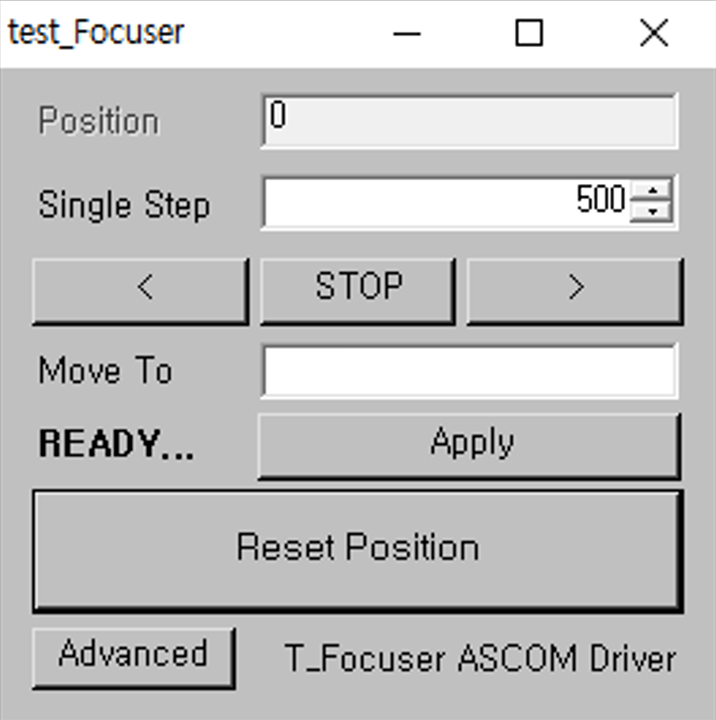
\includegraphics[width=0.75\linewidth]{mainwindow1} 
		\end{center}	
		\caption{Running appearance}
		\label{fig:mainwindow1}
	\end{subfigure}
	\begin{subfigure}{0.5\textwidth}
		\begin{center}			
			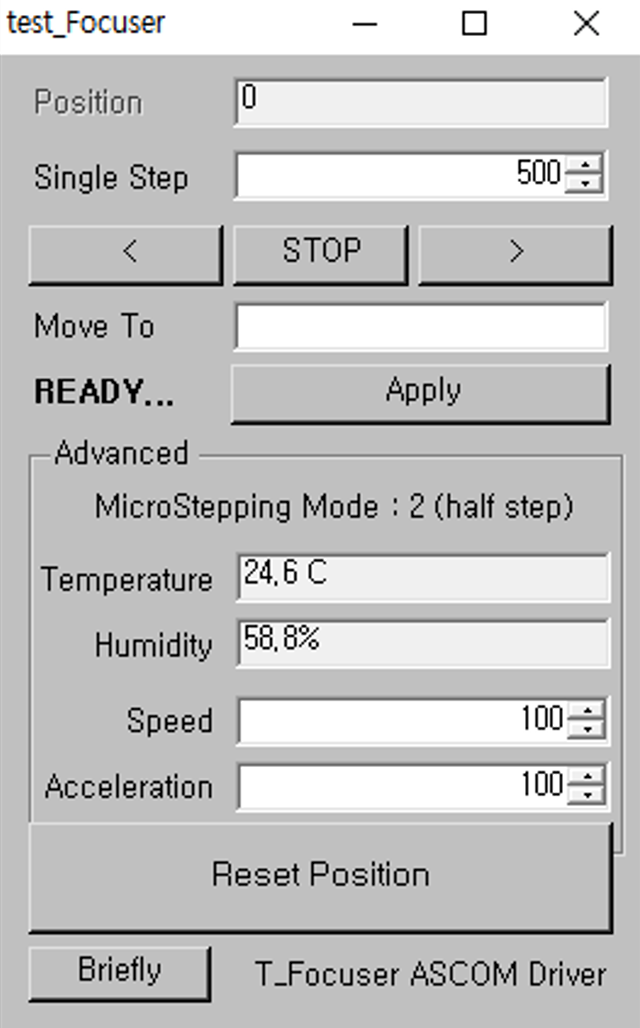
\includegraphics[width=0.75\linewidth]{mainwindow2}
		\end{center}
		\caption{Advanced Running appearance}
		\label{fig:mainwindow2}
	\end{subfigure}
	\caption{MainWindow.cs가 실행되었을 때의 모습}
	\label{fig:mainwindow}
\end{figure}

MainWindow.cs는 펌웨어보다 자유로운 설정이 가능하기 때문에 보다 많은 기능들을 탑재할 수 있었다. 기본적인 기능인 스텝당 움직이는 기능과 더불어 한번에 이동할 single step을 얼마나 크게 할지 직접 설정할 수 있고, 원한다면 모터를 그 상태에서 정지시킬 수도 있으며, 원하는 position을 입력하면 모터가 그 position으로 자동으로 이동하게 할 수도 있다(Move to). 부가적으로는 microstepping과 온도 및 습도를 실시간으로 확인할 수 있으며, 모터가 움직이는 속도와 가속도를 범위 내에서 직접 설정할 수도 있다.

직접 개발한 펌웨어에서도 여러 장점을 찾을 수 있다. Micro Touch제품의 경우, 앞서 나열한 것 외에도 스텝의 초기화 기능이 없기 때문에 모터제어기를 끄고 망원경을 컨트롤하는 등의 변수가 생기면 그 전으로 돌아가기 어렵게 된다. 또한 자신이 원하는 스텝의 위치로 바로 옮기는 것 또한 어려운데, 이 드라이버에서는 원하는 position으로 바로 이동하는 기능도 지원하고 있다. 


